\documentclass[10pt]{amsart}
\usepackage{style}

\title[Homework 2]{Homework 1\\Math 161}
\date{August 31, 2018}
\author{Blake Farman}

\begin{document}
\maketitle

\makenameslot

\begin{thm}
  If a rock is thrown upward on the planet Mars with a velocity of \(10 m/s\), its height in meters \(t\) seconds later is given by \(y = 10t - 1.86t^2\).
  \begin{enumerate}[(a)]
  \item
    Find the average velocity over the given time intervals:
    \begin{enumerate}[(i)]
    \item
      \([1,2]\)
      \vspace{1in}
    \item
      \([1,1.5]\)
      \vspace{1in}
    \item
      \([1,1.1]\)
      \vspace{1in}
    \item
      \([1,1.01]\)
      \newpage
    \item
      \([1,1.001]\)
      \vspace{1in}
    \end{enumerate}
  \item
    Estimate the instantaneous velocity when \(t = 1\).
    \vspace{1in}
  \end{enumerate}
\end{thm}

\begin{thm}
  Explain in your own words what is meant by
  \[\lim_{x \to 2} f(x) = 5.\]
  Is it possible for this statement to be true and yet \(f(2) = 3\)?
  Explain.
  {[Hint: Drawing a picture might help.]}
\end{thm}

\vspace{2in}

\begin{thm}
  Use the given graph of \(f\) to state the value of each quantity, if it exists.
  If it does not exist, explain why.
  \begin{center}
    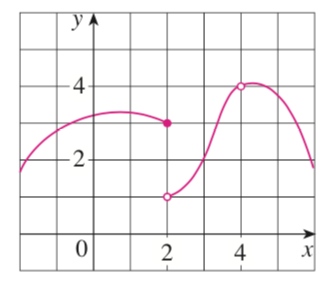
\includegraphics[scale=0.5]{graph}
  \end{center}
  \newpage
  \begin{enumerate}[(a)]
  \item
    \(\lim_{x \to 2^{-}} f(x)\)
    \vspace{1in}
  \item
    \(\lim_{x \to 2^{+}} f(x)\)
    \vspace{1in}
  \item
    \(\lim_{x \to 2} f(x)\)
    \vspace{1in}
  \item
    \(f(2)\)
    \vspace{1in}
  \item
    \(\lim_{x \to 4} f(x)\)
    \vspace{1in}
  \item
    \(f(4)\)
    \vspace{1in}
  \end{enumerate}
\end{thm}
\end{document}

